% =====================================================================
%  CALM Stylized Facts -- Kraken BTC/USD
%  Compile with pdfLaTeX.  Requires the folders  normal/  and  comparison/
%  to sit next to this file (as they do in results/).
% =====================================================================
\documentclass[aspectratio=169,10pt]{beamer}

\usetheme{default}
\useoutertheme{infolines}
\setbeamertemplate{navigation symbols}{}
\setbeamertemplate{caption}[numbered]
\setbeamerfont{caption}{size=\scriptsize}
\setbeamercolor{caption name}{fg=black}
\setbeamerfont{frametitle}{size=\large,series=\bfseries}

\usepackage[T1]{fontenc}
\usepackage{booktabs}
\usepackage{array}
\usepackage{tabularx}
\usepackage{graphicx}
\usepackage{xcolor}
\definecolor{calmblue}{rgb}{0.10,0.28,0.52}
\setbeamercolor{structure}{fg=calmblue}
\usepackage{hyperref}
\hypersetup{colorlinks=true,linkcolor=calmblue,urlcolor=calmblue,citecolor=calmblue}

\graphicspath{{normal/}{comparison/}{./}}

% Weighted X column: widths are proportional and always sum to \textwidth,
% so a table can never overflow the slide however long the text is.
\newcolumntype{L}[1]{>{\raggedright\arraybackslash\hsize=#1\hsize}X}
\newcolumntype{N}{>{\raggedright\arraybackslash}p{0.32cm}}
\setlength{\tabcolsep}{3pt}
\renewcommand{\arraystretch}{1.05}

\title[CALM Stylized Facts]{CALM Stylized Facts}
\subtitle{Kraken BTC/USD L3 Evidence for TCA Simulation}
\author{Kai Liu}
\date{September 9, 2026}

\begin{document}

\begin{frame}[plain]
  \titlepage
\end{frame}
\begin{frame}{Scope and Priority Labels}
\footnotesize
\textbf{Goal.} Calibrate and validate a limit-order-book simulator whose output is a
\emph{liquidation impact} estimate. Priority follows how directly a fact changes that estimate.

\medskip
\begin{tabularx}{\textwidth}{@{}p{1.1cm}X@{}}
\toprule
\textbf{P0} & \textbf{You configure it, or it is the answer.} Either a parameter typed into the
simulator, or the number the simulator must reproduce. Seven facts. Wrong here and the liquidation
estimate is wrong by construction. \\[2pt]
\textbf{P1} & \textbf{It must emerge correctly.} Not set directly, but if the simulated market fails
to reproduce it the cost number cannot be trusted. Six facts. \\[2pt]
\textbf{P2} & \textbf{Realism and second order.} Improves face validity and matters for
multi-liquidation cascade scenarios; little effect on a single liquidation cost. Six facts. \\
\bottomrule
\end{tabularx}

\medskip
\textbf{Calibration budget.} Nineteen facts is more than one project can calibrate. If effort is
constrained, the ten-fact core is \textbf{all of P0 plus facts 8, 9 and 10} --- the flow-to-price
transfer, the per-order impact kernel, and order-sign memory.

\medskip
\textbf{Why this ordering.} Taken from the capstone proposal: the deliverable is a discrete-event
LOB simulator with market-maker, taker and liquidation agents, used to quantify a market impact
coefficient for TWAP / VWAP / instant liquidation under different liquidity regimes, and to answer
two named questions --- \emph{liquidity capacity thresholds} and \emph{spread recovery times}.
Facts that feed those two answers, or that set a named agent parameter, are P0.

\medskip
\textbf{Measurability.} Facts 1--3 have no parent-order labels in public data and are measured
through a \emph{proxy}; they are validation targets, not calibration inputs.
\end{frame}
\begin{frame}{Proposal Requirements Mapped to Facts}
\scriptsize
\begin{tabularx}{\textwidth}{@{}L{0.85}L{1.15}@{}}
\toprule
\textbf{Proposal component} & \textbf{Facts that calibrate or validate it} \\
\midrule
Taker bots, specified as \emph{Poisson arrival times} &
19 arrivals (\textbf{Poisson is rejected}: Fano 3 at 1\,s rising to 28 at 300\,s),
16 order sizes, 10 sign memory \\[2pt]
Market makers, Avellaneda--Stoikov with inventory &
6 spread, 13 queue imbalance, 20 depth profile, 7 resiliency \\[2pt]
Liquidation bot: TWAP vs VWAP vs instant &
1--3 impact and its duration exponent $\gamma$, 7 recovery between slices,
22 the market's own execution clock \\[2pt]
Market impact coefficient under liquidity regimes &
8 OFI, 9 response function, 5 cost curve; normal against stress in the appendix \\[2pt]
Named question: \emph{liquidity capacity thresholds} & 5 cost curve and visible depth \\[2pt]
Named question: \emph{spread recovery times} & 7 resiliency \\[2pt]
Configurable parameters named in the proposal:
\emph{order arrival rates, book depth profiles} & 19 and 20, both P0 for exactly this reason \\[2pt]
Cascading liquidations & 7 resiliency, 14 volatility clustering, 11 diffusivity \\
\bottomrule
\end{tabularx}
\end{frame}
\begin{frame}{Data, Reconstruction and Proxy}
\footnotesize
\textbf{Period.} Normal week: 18--24 July 2026 (UTC), 167.95 measured hours. One extra calendar
day precedes it purely to warm the book up.

\medskip
\textbf{Feed.} Kraken BTC/USD \textbf{L3}: per-order add / modify / delete plus trade prints, top
100 price levels per side, tick $=0.1$ USD.
\begin{itemize}\itemsep1pt
  \item 85.6M raw rows $\rightarrow$ 61.7M packets $\rightarrow$ 161{,}702 aggressive orders,
        4.49M top-of-book events, 396{,}688 fills.
  \item The window is depth-limited and scrolls out silently, so 23.4M level evictions are applied
        by the reconstruction; book state is read only at packet boundaries.
  \item Book and trade channels are separate subscriptions, so an order's pre-trade book is taken
        on \emph{exchange} time. Aggressor-side consistency: 0.992 exchange-aligned against 0.777
        receipt-aligned.
  \item 65 exchange snapshot blocks serve as out-of-sample checks; median reconstruction error
        0 ticks.
\end{itemize}

\medskip
\textbf{Metaorder proxy (Facts 1--3).} Public data carries no parent labels. Each aggressive order
is assigned at random to one of $N=6$ synthetic traders; a metaorder is a run of same-signed trades
from one trader within a UTC day. Scales are per day: $V_D$ = daily volume,
$\sigma_D=(\max p-\min p)/p_0$.
Method: \href{https://arxiv.org/abs/2503.18199}{Maitrier, Loeper \& Bouchaud (2025a)}, Algorithms
1--2. Three seeds are run; only $N=6$ is reported here.

\medskip
\textbf{Convention.} Signed impacts are kept throughout. No positive-impact pre-filter is applied,
because selecting on the outcome changes the estimand.
\end{frame}
\begin{frame}{P0 --- Configure It, or It Is the Answer (1/2)}
\scriptsize
\begin{tabularx}{\textwidth}{@{}N L{0.62} L{1.02} L{1.10} L{1.26}@{}}
\toprule
\textbf{\#} & \textbf{Fact} & \textbf{Definition} & \textbf{Why prioritised} & \textbf{Extant finding and source} \\
\midrule
1 & Concave metaorder impact & $I(Q)/\sigma_D$ against $Q/V_D$ at completion. &
\textbf{It is the deliverable.} The proposal's ``market impact coefficient'' is this curve. &
Square-root law on Bitcoin over six decades.
\href{https://arxiv.org/abs/1412.4503}{Donier \& Bonart (2015)}. \\[3pt]
5 & Liquidity cost and depth & Virtual market-order VWAP cost and cumulative visible depth. &
\textbf{Named deliverable:} the \emph{liquidity capacity threshold}. Also bounds what one order can
absorb. & Cost rises with size; book roughly symmetric. \href{https://www.mdpi.com/1911-8074/12/1/25}{Schnaubelt et al.\ (2019)}. \\[3pt]
7 & Liquidity resiliency & Recovery of spread, depth and cost after a large aggressive order. &
\textbf{Named deliverable:} the \emph{spread recovery time}. Sets safe spacing between slices. &
Spread recovers over a few seconds. \href{https://www.mdpi.com/1911-8074/12/1/25}{Schnaubelt et al.\ (2019)}; Obizhaeva \& Wang (2013). \\[3pt]
19 & Event arrivals and clustering & Interarrival distribution and count dispersion. &
\textbf{Named configurable parameter} (arrival rates), and the proposal's Poisson assumption is
rejected by the data. & Strongly over-dispersed; self-exciting models are the standard fit.
Bacry, Mastromatteo \& Muzy (2015). \\
\bottomrule
\end{tabularx}
\end{frame}
\begin{frame}{Facts 1--3: Metaorder Impact, $N=6$ Proxy}
\begin{figure}
\centering
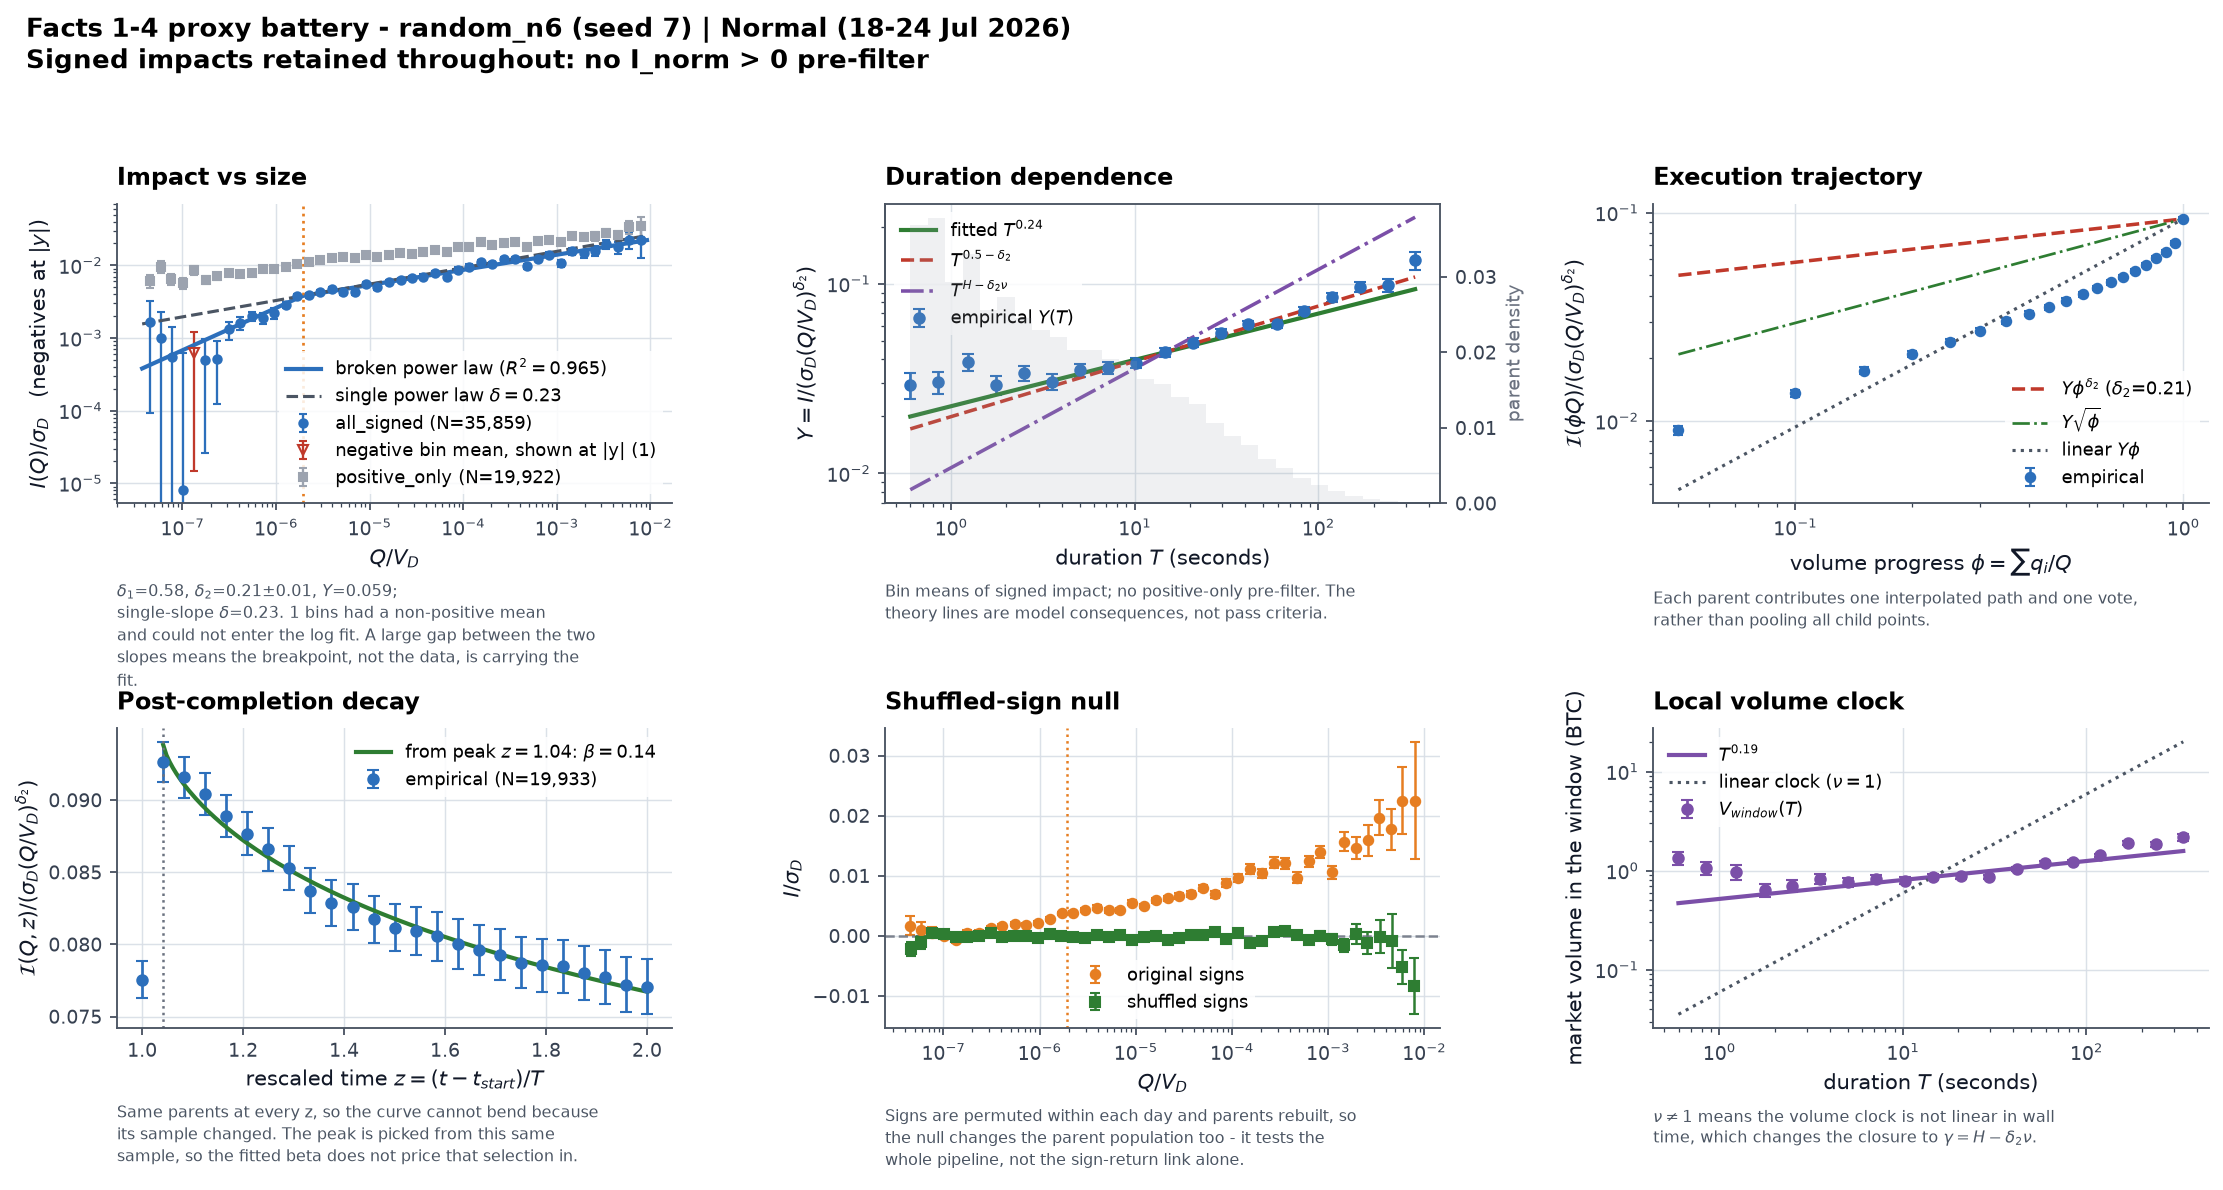
\includegraphics[width=\textwidth,height=0.74\textheight,keepaspectratio]{fact_meta_nb_battery_random_n6_seed7__normal}
\caption{Same figure also carries facts 2 and 3, quantified two slides on. Impact is concave in size but far below square root: $\delta_2=0.21$
(single-slope $\delta=0.23$), $Y=0.061$. Decay exponent $\beta=0.14$. The execution trajectory is
linear rather than concave, $y(0.5)/y(1)=0.39$ against $0.71$ for $\sqrt{\phi}$.}
\end{figure}
\end{frame}
\begin{frame}{Fact 5: Liquidity Cost and Visible Depth}
\begin{figure}
\centering

\includegraphics[width=\textwidth,height=0.74\textheight,keepaspectratio]{fact05_liquidity_cost_and_depth__normal}
\caption{Virtual market-order cost rises steeply with size; cumulative visible depth saturates
around 20\,bps, which is where the 100-level publication window ends.}
\end{figure}
\end{frame}
\begin{frame}{Fact 7: Liquidity Resiliency}
\begin{figure}
\centering

\includegraphics[width=\textwidth,height=0.74\textheight,keepaspectratio]{fact07_resiliency__normal}
\caption{After large aggressive orders, spread and depth recover on different timescales.}
\end{figure}
\end{frame}
\begin{frame}{Fact 19: Event Arrivals and Clustering}
\begin{figure}
\centering
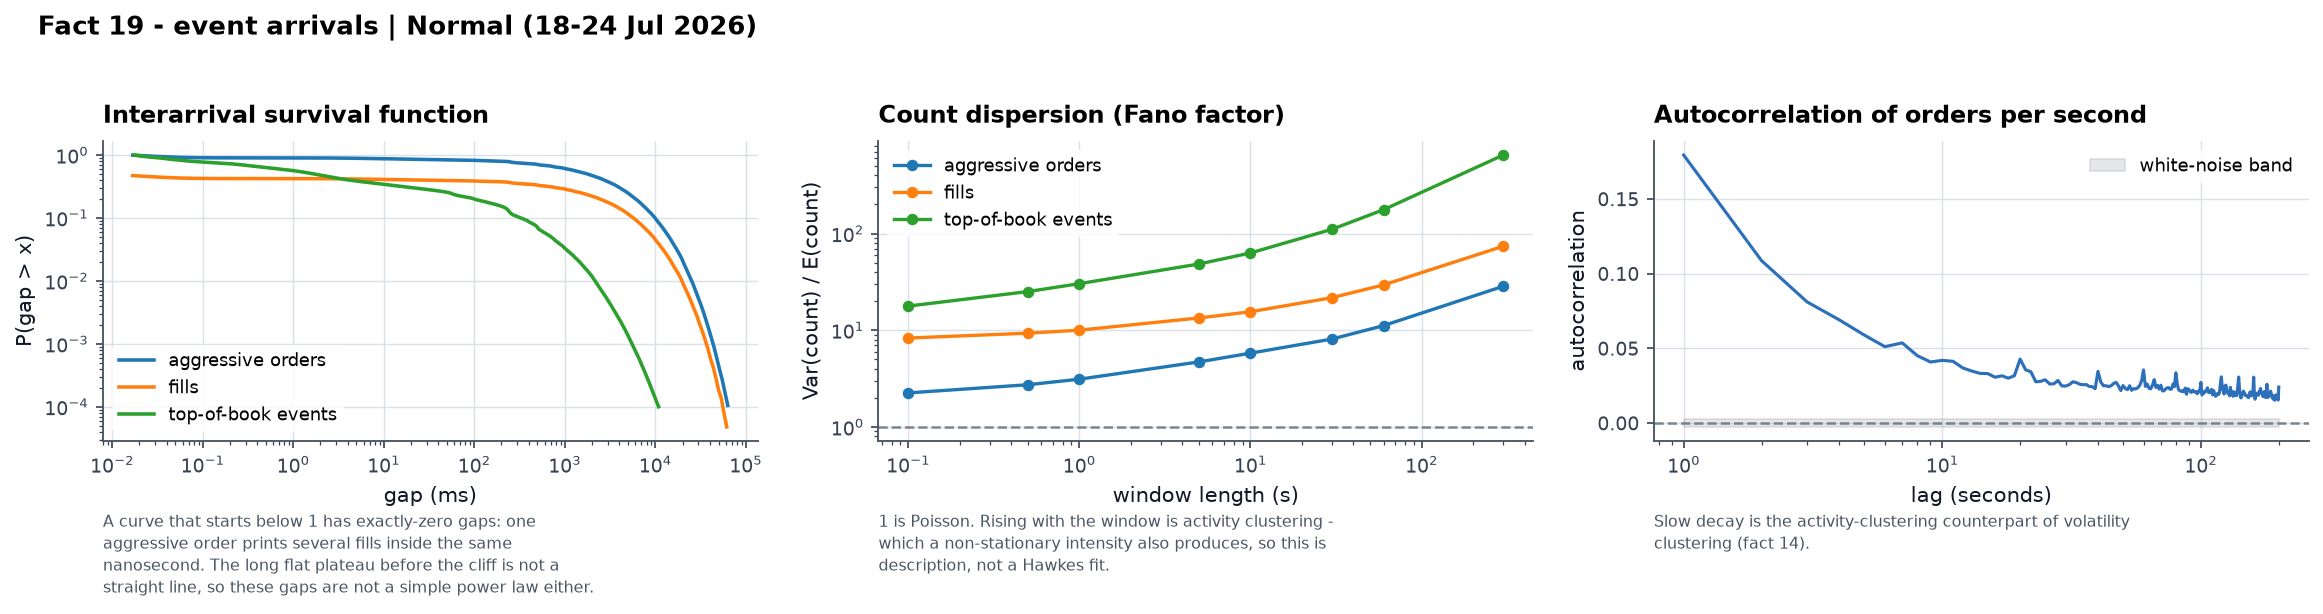
\includegraphics[width=\textwidth,height=0.74\textheight,keepaspectratio]{fact19_arrivals__normal}
\caption{Mean interarrival is 3.74\,s for aggressive orders and 135\,ms for top-of-book events.
The Fano factor rises from 3 at 1\,s to 28 at 300\,s: strongly over-dispersed against Poisson.}
\end{figure}
\end{frame}
\begin{frame}{P0 --- Configure It, or It Is the Answer (2/2)}
\scriptsize
\begin{tabularx}{\textwidth}{@{}N L{0.62} L{1.02} L{1.10} L{1.26}@{}}
\toprule
\textbf{\#} & \textbf{Fact} & \textbf{Definition} & \textbf{Why prioritised} & \textbf{Extant finding and source} \\
\midrule
20 & Book shape & L1 depth distribution and depth per level away from the touch. &
\textbf{Named configurable parameter} (depth profiles). Sets how far a liquidation walks the book. &
Depth grows away from the touch; sides roughly symmetric. \href{https://www.mdpi.com/1911-8074/12/1/25}{Schnaubelt et al.\ (2019)}. \\[3pt]
16 & Trade-size distribution & Distribution of aggressive-order and fill sizes. &
\textbf{Agent parameter:} taker-bot order sizes. The tail governs how often the queue clears in one
hit. & Heavy upper tail plus clustering on round sizes. \href{https://www.mdpi.com/1911-8074/12/1/25}{Schnaubelt et al.\ (2019)}. \\[3pt]
6 & Spread distribution & Distribution of the quoted spread and its state dependence. &
\textbf{Agent parameter:} the maker's quoting width, and the unavoidable cost floor paid on every
child order. & Tight with a heavy right tail; state dependent. \href{https://www.mdpi.com/1911-8074/12/1/25}{Schnaubelt et al.\ (2019)}. \\
\bottomrule
\end{tabularx}
\end{frame}
\begin{frame}{Fact 20: Book Shape}
\begin{figure}
\centering
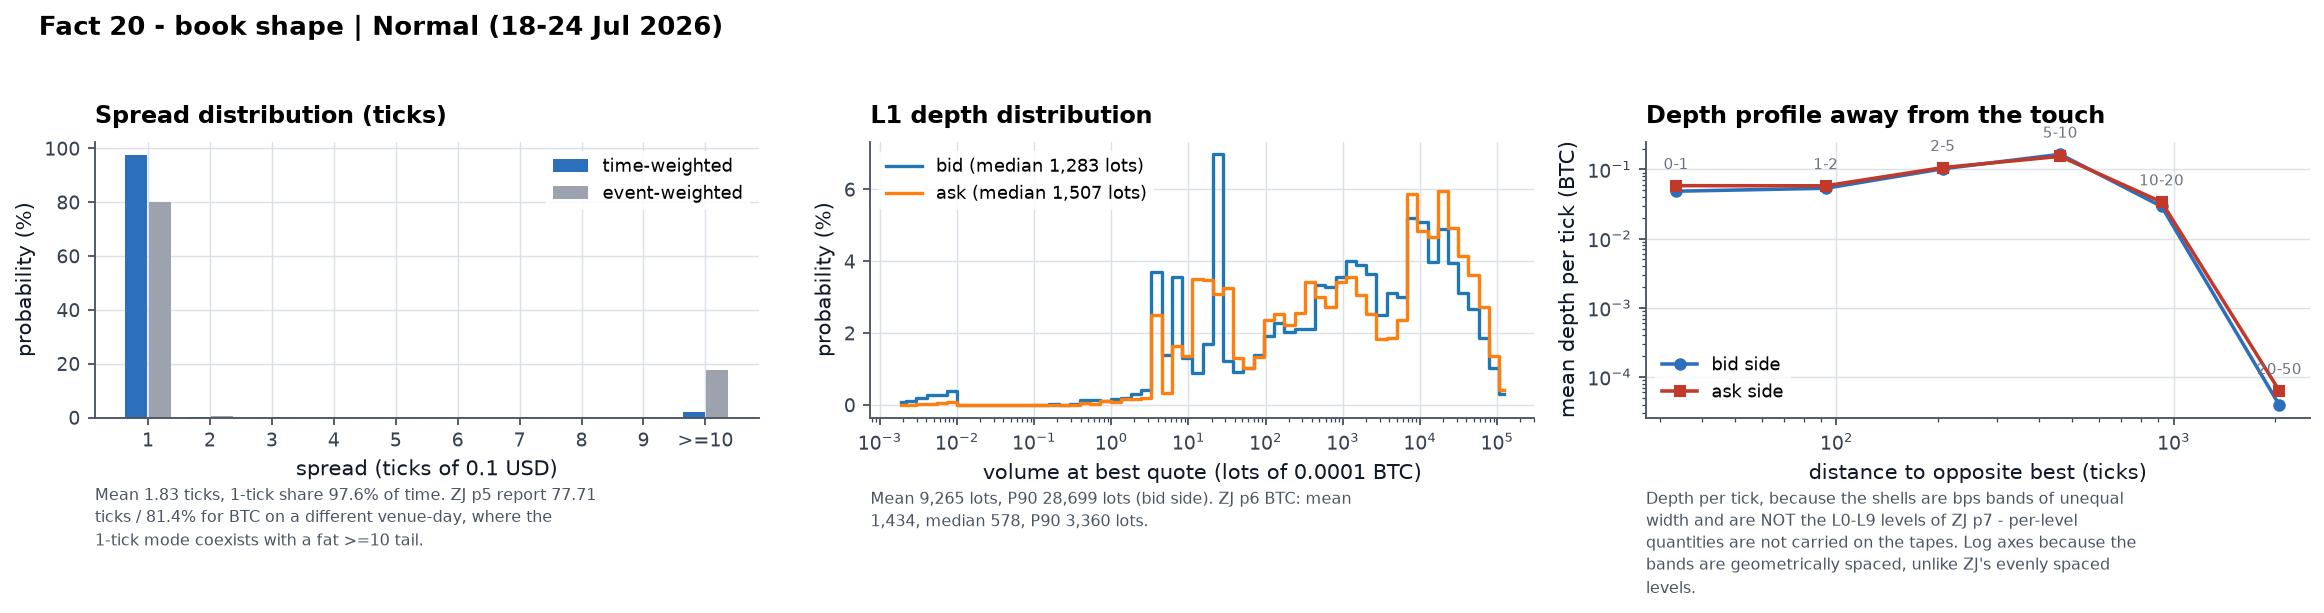
\includegraphics[width=\textwidth,height=0.74\textheight,keepaspectratio]{fact20_book_shape__normal}
\caption{The book is one tick wide 97.6\% of the \emph{time} but only 80.2\% of \emph{updates}:
wide spreads are short-lived (16\,ms mean dwell against 164\,ms at one tick).}
\end{figure}
\end{frame}
\begin{frame}{Fact 20: L1 Depth and Volume Profile}
\begin{figure}
\centering
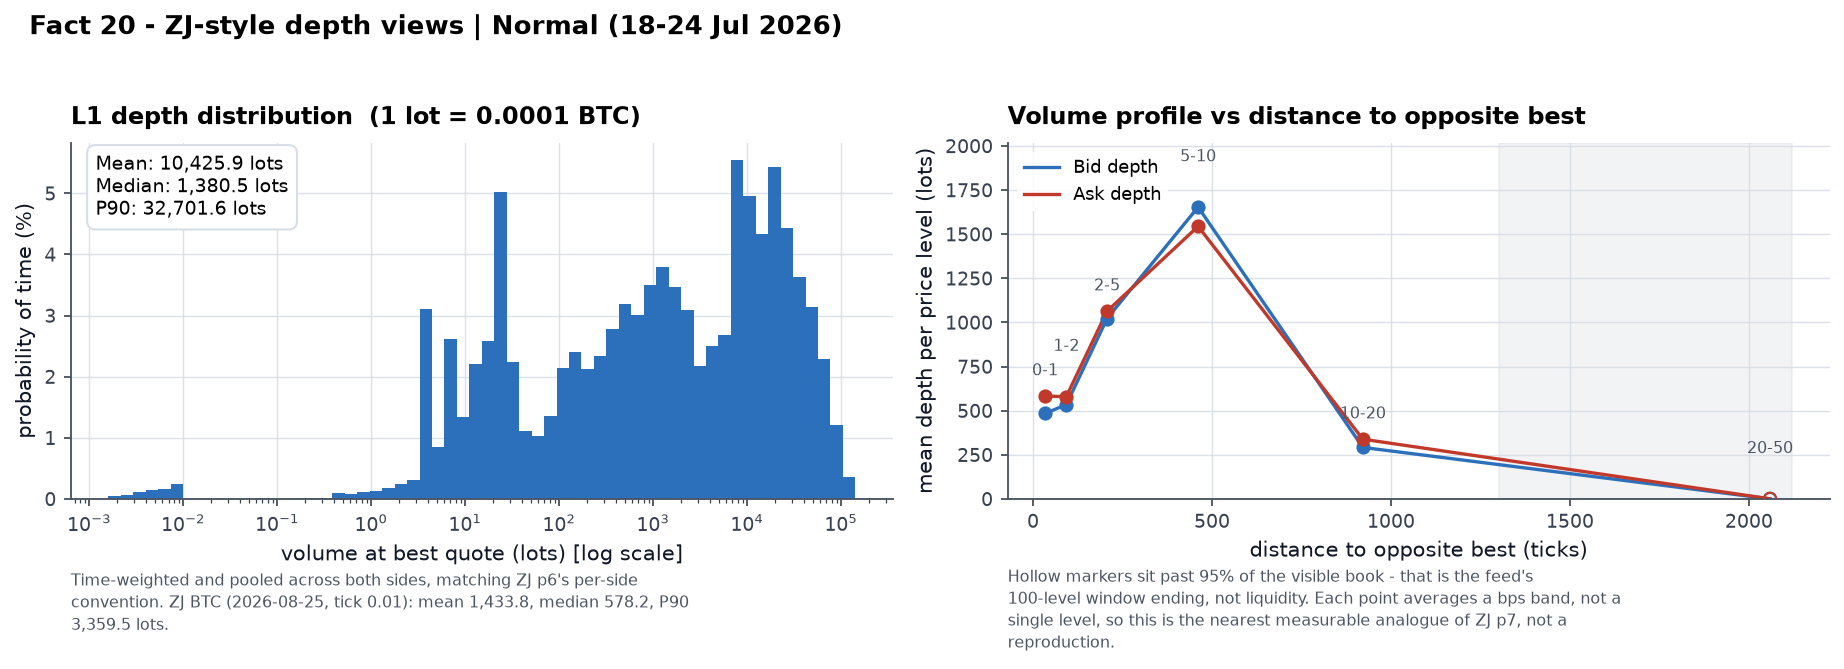
\includegraphics[width=\textwidth,height=0.74\textheight,keepaspectratio]{fact20_zj_style_depth__normal}
\caption{L1 depth median 1{,}380 lots (1 lot $=10^{-4}$ BTC). Depth per price level rises away from
the touch and then collapses; hollow markers are the 100-level publication window ending, not the
market thinning.}
\end{figure}
\end{frame}
\begin{frame}{Fact 16: Trade-Size Distribution}
\begin{figure}
\centering

\includegraphics[width=\textwidth,height=0.74\textheight,keepaspectratio]{fact16_trade_size__normal}
\caption{Aggressive-order sizes have a heavy upper tail: p99/median $\approx700\times$ and the
largest 1\% of orders carry about 40\% of all volume.}
\end{figure}
\end{frame}
\begin{frame}{Fact 6: Spread Distribution and State Dependence}
\begin{figure}
\centering

\includegraphics[width=\textwidth,height=0.74\textheight,keepaspectratio]{fact06_spread_distribution__normal}
\caption{Spreads are tight and quantised: one tick is $\approx0.015$\,bps at these prices, so the
comb of spikes is 1, 2, 3 ticks and the gaps between are real.}
\end{figure}
\end{frame}
\begin{frame}{P1 --- Must Emerge Correctly (1/2)}
\scriptsize
\begin{tabularx}{\textwidth}{@{}N L{0.62} L{1.02} L{1.10} L{1.26}@{}}
\toprule
\textbf{\#} & \textbf{Fact} & \textbf{Definition} & \textbf{Why prioritised} & \textbf{Extant finding and source} \\
\midrule
8 & Order-flow imbalance & Mid-price change regressed on OFI over fixed windows. &
The flow-to-price transfer function. If the simulated book does not reproduce it, the shock
propagates at the wrong rate. & Mid changes approximately linear in OFI, coefficient falling with
depth. \href{https://arxiv.org/abs/1011.6402}{Cont, Kukanov \& Stoikov (2014)}. \\[3pt]
9 & Trade response $\mathcal{R}(\ell)$ & $\langle \epsilon_t (m_{t+\ell}-m_t)\rangle$ in trade
time. & The per-order impact kernel. Metaorder cost is this aggregated over a schedule, so it must
come out right first. & Rises with $\ell$ and settles despite persistent flow.
\href{https://arxiv.org/abs/cond-mat/0307332}{Bouchaud et al.\ (2004)}. \\[3pt]
10 & Order-sign long memory & $C(\ell)=\mathrm{Cov}(\epsilon_t,\epsilon_{t+\ell})\sim
\ell^{-\gamma}$. & If simulated flow comes out i.i.d.\ the book refills too easily and liquidation
cost is \emph{understated}. & Power-law decay with $\gamma<1$, from order splitting.
\href{https://arxiv.org/abs/cond-mat/0311053}{Lillo \& Farmer (2004)}. \\
\bottomrule
\end{tabularx}
\end{frame}
\begin{frame}{Fact 8: Order-Flow Imbalance, Event Time}
\begin{figure}
\centering

\includegraphics[width=\textwidth,height=0.74\textheight,keepaspectratio]{fact08_ofi_response__normal}
\caption{Mid change is close to linear in OFI over 50-quote-event blocks, and the impact
coefficient falls as depth rises, as Cont, Kukanov \& Stoikov predict.}
\end{figure}
\end{frame}
\begin{frame}{Fact 8b: OFI versus TFI, Clock Windows}
\begin{figure}
\centering
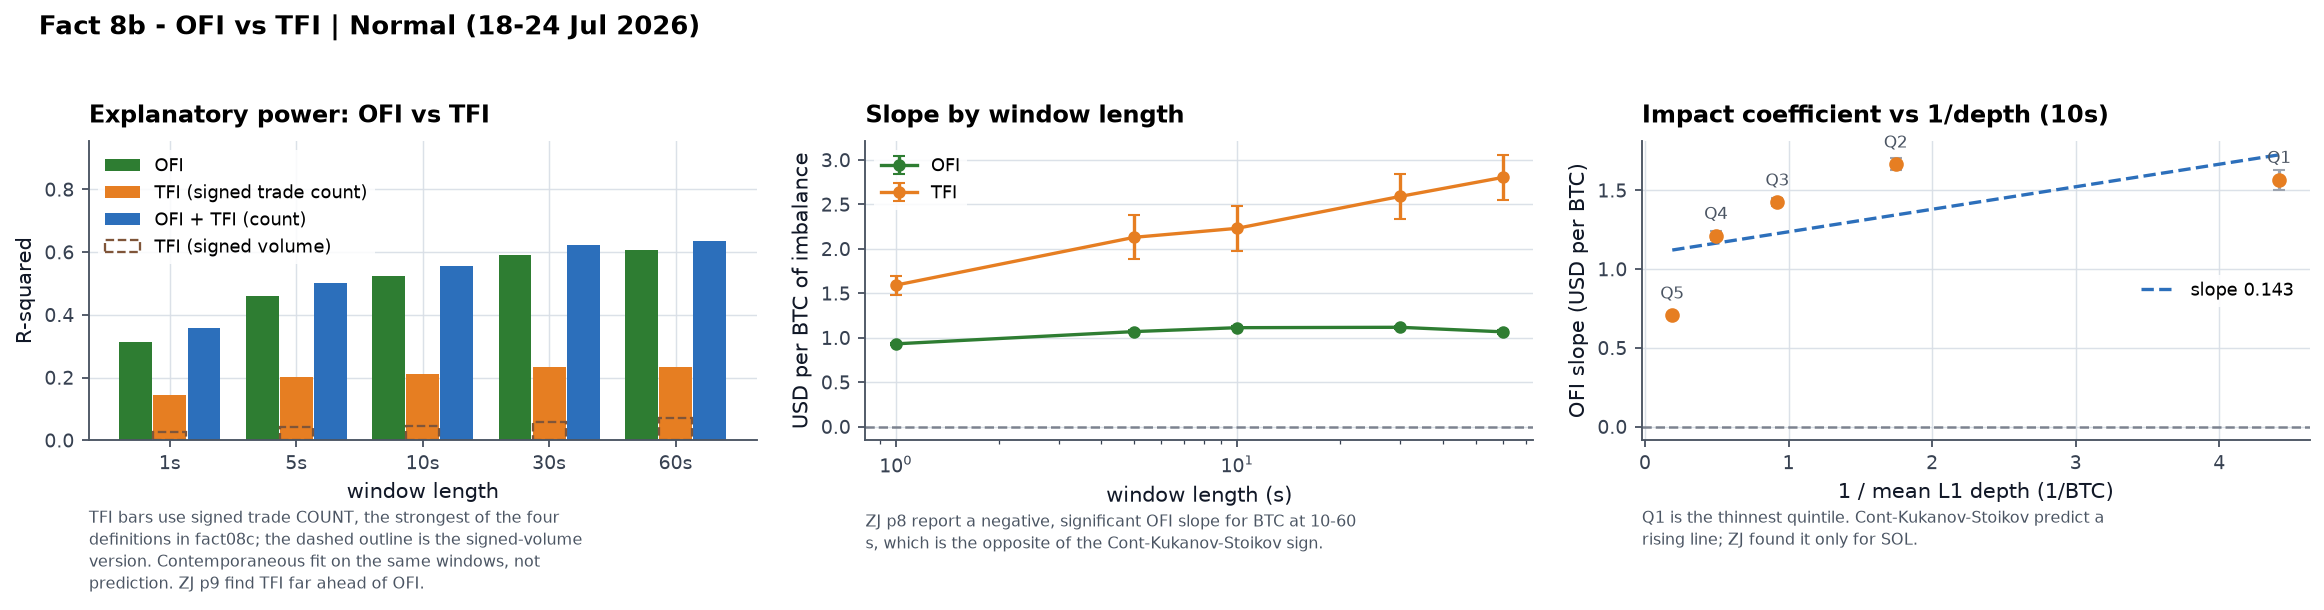
\includegraphics[width=\textwidth,height=0.74\textheight,keepaspectratio]{fact08b_ofi_tfi__normal}
\caption{OFI explains $R^2=0.52$ at 10\,s against $0.21$ for the strongest trade-flow definition
(signed trade count) and $0.05$ for signed volume. The slope is positive and falls monotonically
across depth quintiles.}
\end{figure}
\end{frame}
\begin{frame}{Fact 8c: Real-Time OFI across Horizons}
\begin{figure}
\centering
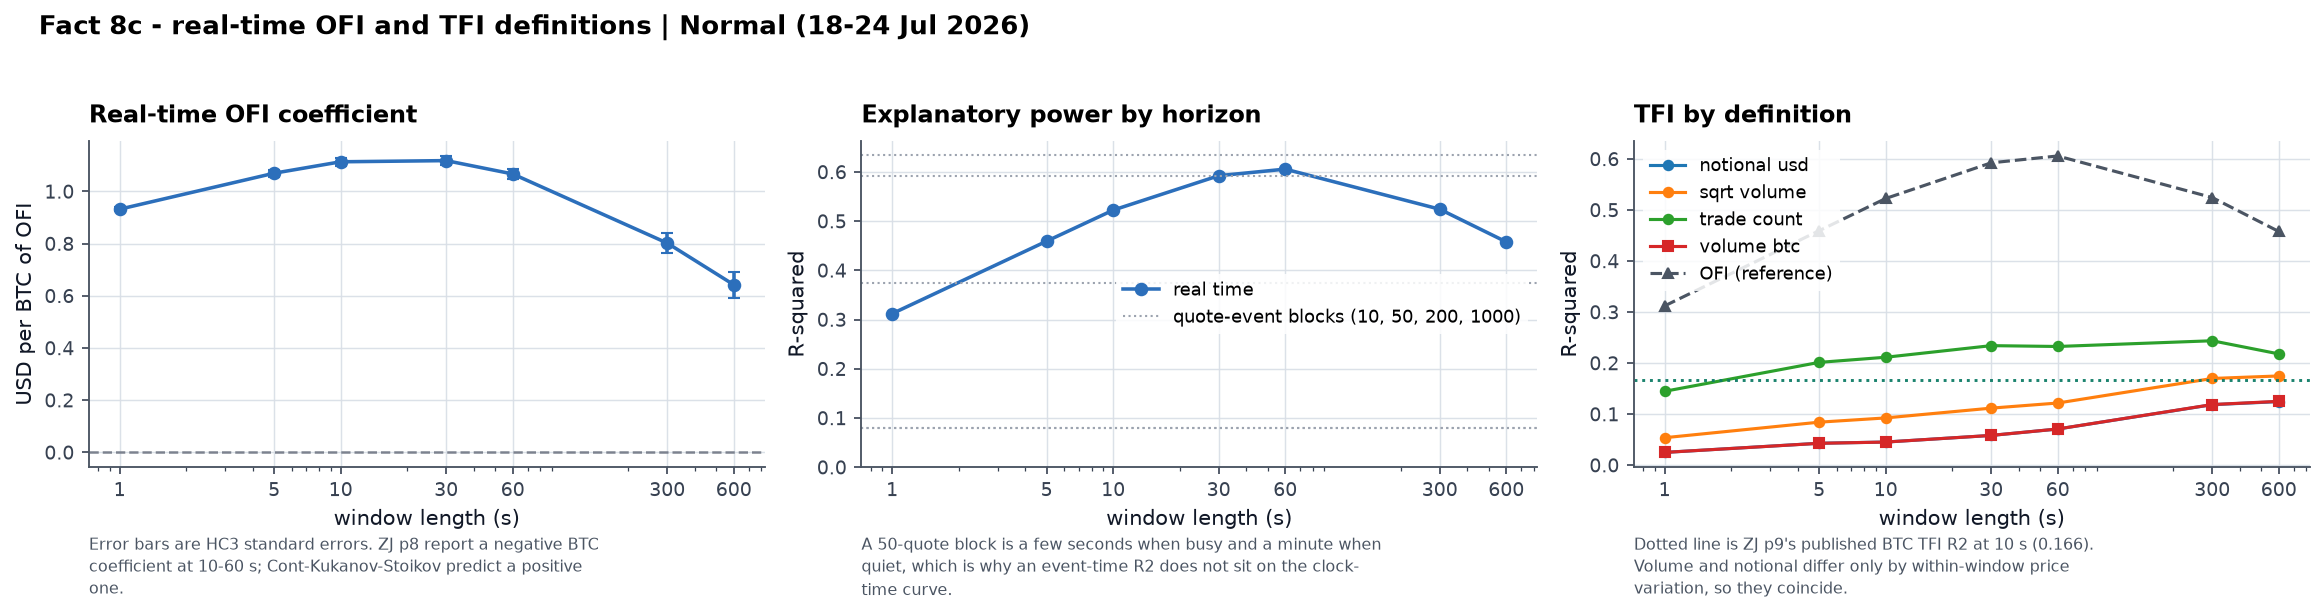
\includegraphics[width=\textwidth,height=0.74\textheight,keepaspectratio]{fact08c_realtime_ofi_tfi__normal}
\caption{Explanatory power peaks near 60\,s ($R^2=0.61$) and decays by 600\,s ($0.46$); the slope
peaks at $+1.11$ USD per BTC at 10--30\,s. The relation is a roughly one-minute phenomenon.}
\end{figure}
\end{frame}
\begin{frame}{Fact 9: Trade Response Function}
\begin{figure}
\centering

\includegraphics[width=\textwidth,height=0.74\textheight,keepaspectratio]{fact09_trade_response__normal}
\caption{Signed aggressive orders move the mid in their own direction, growing slowly with lag
rather than jumping and reverting.}
\end{figure}
\end{frame}
\begin{frame}{Fact 9: Conditional Response $\mathcal{R}(\ell)$, $\mathcal{R}(v,1)$, $\mathcal{R}^{\pm}(1)$}
\begin{figure}
\centering
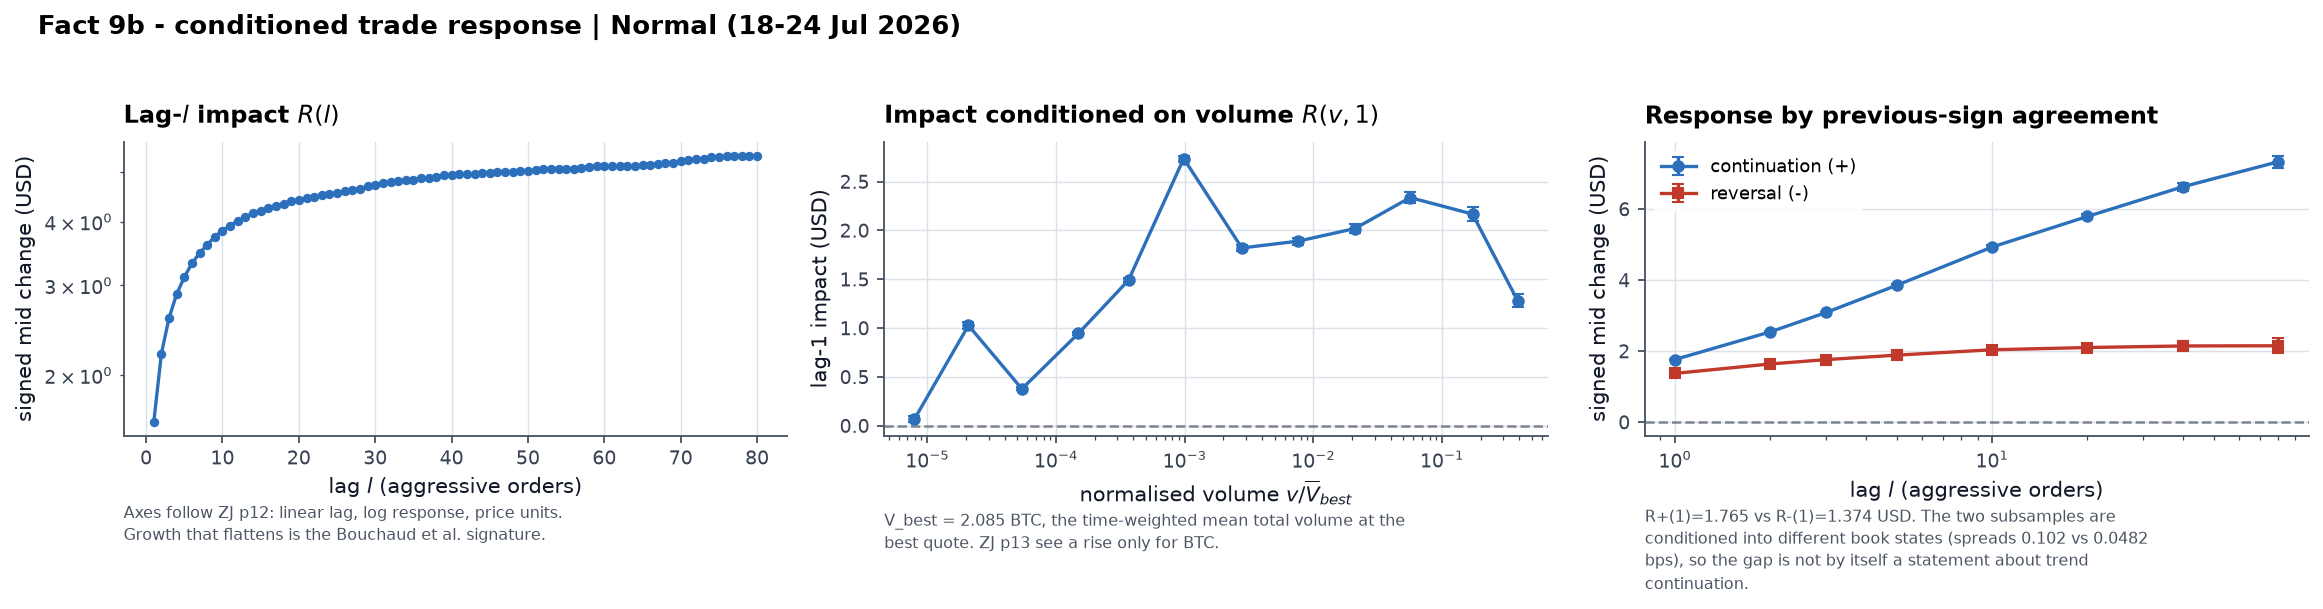
\includegraphics[width=\textwidth,height=0.74\textheight,keepaspectratio]{fact09b_conditional_response__normal}
\caption{$\mathcal{R}(\ell)$ rises from 1.62 to 5.39 USD over 80 orders. $\mathcal{R}^{+}(1)=1.77$
against $\mathcal{R}^{-}(1)=1.37$ USD, but the two subsamples face different spreads (0.102 against
0.048\,bps); scaled by the spread faced, the ordering reverses.}
\end{figure}
\end{frame}
\begin{frame}{Fact 10: Order-Sign Long Memory}
\begin{figure}
\centering

\includegraphics[width=\textwidth,height=0.74\textheight,keepaspectratio]{fact10_sign_memory__normal}
\caption{Signs decay as a power law with $\gamma=0.54$ over lags 10--1000; $C(1)=0.23$ and
$C(100)=0.011$, still above the noise floor.}
\end{figure}
\end{frame}
\begin{frame}{P1 --- Must Emerge Correctly (2/2)}
\scriptsize
\begin{tabularx}{\textwidth}{@{}N L{0.62} L{1.02} L{1.10} L{1.26}@{}}
\toprule
\textbf{\#} & \textbf{Fact} & \textbf{Definition} & \textbf{Why prioritised} & \textbf{Extant finding and source} \\
\midrule
2 & Impact trajectory and duration & Impact against executed fraction $\phi$ and execution time
$T$. & Decides whether slowing down helps. TWAP beats an instant order only if impact depends on
$T$. & Concave $\propto\sqrt{\phi}$; impact roughly independent of $T$.
\href{https://arxiv.org/abs/2503.18199}{Maitrier et al.\ (2025a)}. \\[3pt]
3 & Post-execution decay & Relaxation of impact after the last child order. &
Splits cost into temporary and permanent. Only the permanent part propagates into a cascade. &
Decays toward a permanent level; propagator picture.
\href{https://arxiv.org/abs/cond-mat/0307332}{Bouchaud et al.\ (2004)}. \\[3pt]
11 & Diffusive prices under persistent flow & Variance ratio and return autocorrelation across
clocks. & No-free-money check. Persistent flow must not produce arbitrageable drift, or the
simulator is exploitable. & Returns near-unpredictable despite persistent signs.
\href{https://academic.oup.com/rfs/article/1/1/41/1601244}{Lo \& MacKinlay (1988)}. \\
\bottomrule
\end{tabularx}
\end{frame}
\begin{frame}{Facts 2 and 3: Trajectory and Decay, $N=6$ Proxy}
\footnotesize
\begin{tabularx}{\textwidth}{@{}L{1.35}L{0.75}L{0.90}@{}}
\toprule
\textbf{Quantity} & \textbf{Measured} & \textbf{Reference} \\
\midrule
\multicolumn{3}{@{}l}{\textbf{Fact 2 --- trajectory in executed volume $\phi$}} \\
$y(0.25)/y(1)$                                & 0.27  & --- \\
$y(0.50)/y(1)$                                & 0.39  & 0.87 concave $\phi^{\delta_2}$; 0.71 $\sqrt{\phi}$; 0.50 linear \\
$y(0.75)/y(1)$                                & 0.54  & --- \\
\midrule
\multicolumn{3}{@{}l}{\textbf{Fact 2 --- dependence on execution time $T$}} \\
Duration exponent $\gamma$                    & 0.247 & 0.288 from $0.5-\delta_2$ \\
                                              &       & 0.522 from $H-\delta_2\nu$ \\
Volume-clock exponent $\nu$                   & 0.194 & 1.0 for a linear clock \\
\midrule
\multicolumn{3}{@{}l}{\textbf{Fact 3 --- decay after completion, rescaled clock $z=t/T$}} \\
Propagator exponent $\beta$                   & 0.142 & 0.114 reported for DOGE in the notebook \\
Peak location $z$                             & 1.04  & 1.0 if impact peaks at completion \\
Fit $R^2$ from the peak                       & 0.986 & --- \\
\bottomrule
\end{tabularx}

\medskip
\scriptsize
The trajectory is \emph{linear}, not concave. That is a property of the proxy on this instrument,
not of the market: the median synthetic parent holds 66\% of its volume in a single child, so the
volume axis is barely resolved. Reported as measured, without correction.
\end{frame}

\begin{frame}{Fact 11: Diffusivity under Persistent Flow}
\begin{figure}
\centering

\includegraphics[width=\textwidth,height=0.74\textheight,keepaspectratio]{fact11_diffusion__normal}
\caption{Variance ratio is 0.90 at short quote-event lags (bid-ask bounce) but 2.66 at
$k\!\ge\!100$; on 60\,s bars it is 0.94. Adaptive liquidity does not fully absorb the persistent
flow at minute scales.}
\end{figure}
\end{frame}
\begin{frame}{P2 --- Realism and Second Order (1/2)}
\scriptsize
\begin{tabularx}{\textwidth}{@{}N L{0.62} L{1.02} L{1.10} L{1.26}@{}}
\toprule
\textbf{\#} & \textbf{Fact} & \textbf{Definition} & \textbf{Why prioritised} & \textbf{Extant finding and source} \\
\midrule
13 & Queue-imbalance predictability & $(q_b-q_a)/(q_b+q_a)$ against the next price move. &
The skew signal an Avellaneda--Stoikov maker can quote on. Improves maker realism; does not move
the cost estimate. & Predicts the one-tick-ahead move.
\href{https://arxiv.org/abs/1512.03492}{Gould \& Bonart (2016)}. \\[3pt]
14 & Volatility clustering & Autocorrelation of absolute returns across horizons. &
The feedback channel for \emph{cascading} liquidations. Second order for a single liquidation,
first order if cascades are simulated. & Slowly decaying at minute and hour scales.
\href{https://www.mdpi.com/1911-8074/12/1/25}{Schnaubelt et al.\ (2019)}; Cont (2001). \\[3pt]
12 & Selective liquidity taking & Book state in the minutes before unusually large aggressive
orders. & A forced liquidation cannot time its entry, so this only bounds the gap against voluntary
trading. & Large trades are timed into favourable liquidity 2--3 minutes ahead. \href{https://www.mdpi.com/1911-8074/12/1/25}{Schnaubelt et al.\ (2019)}. \\
\bottomrule
\end{tabularx}
\end{frame}
\begin{frame}{Fact 13: Queue-Imbalance Predictability}
\begin{figure}
\centering

\includegraphics[width=\textwidth,height=0.74\textheight,keepaspectratio]{fact13_queue_imbalance__normal}
\caption{Queue imbalance carries directional information about the next price move; accuracy is
reported against the majority-class baseline and with coverage.}
\end{figure}
\end{frame}
\begin{frame}{Fact 14: Volatility Clustering}
\begin{figure}
\centering

\includegraphics[width=\textwidth,height=0.74\textheight,keepaspectratio]{fact14_volatility_clustering__normal}
\caption{Absolute returns stay autocorrelated far beyond the return autocorrelation itself, at both
minute and hour scales.}
\end{figure}
\end{frame}
\begin{frame}{Fact 12: Selective Liquidity Taking}
\begin{figure}
\centering

\includegraphics[width=\textwidth,height=0.74\textheight,keepaspectratio]{fact12_selective_liquidity__normal}
\caption{Book state in the minutes before unusually large aggressive orders, against a
time-weighted baseline.}
\end{figure}
\end{frame}
\begin{frame}{P2 --- Realism and Second Order (2/2)}
\scriptsize
\begin{tabularx}{\textwidth}{@{}N L{0.62} L{1.02} L{1.10} L{1.26}@{}}
\toprule
\textbf{\#} & \textbf{Fact} & \textbf{Definition} & \textbf{Why prioritised} & \textbf{Extant finding and source} \\
\midrule
18 & Price-diffusion scaling & $\sigma(\tau)=\mathrm{std}(r_\tau)\sim\tau^{H}$ over
0.2--60\,s. & Fixes the volatility scale that impact is quoted in. Affects units, not the mechanism. &
$H\approx0.5$ over the diffusive range, flatter at sub-second lags.
\href{https://academic.oup.com/rfs/article/1/1/41/1601244}{Lo \& MacKinlay (1988)}. \\[3pt]
22 & Order-timing regularity & Periodicity of arrival times and wall-clock anchoring. &
TWAP is itself a clock and the market has one too, so scheduled children can meet a crowd. Refines
timing, not size. & Activity concentrates at one-second intervals
(\href{https://onlinelibrary.wiley.com/doi/10.1111/fima.12405}{Muravyev \& Picard, 2022}); spot BTC
surges in the first second of the minute
(\href{https://www.tandfonline.com/doi/full/10.1080/13504851.2026.2617499}{Shynkevich, 2026}). \\[3pt]
17 & 24/7 intraday structure & Hourly profile of volume, spread and depth. &
Face validity only: a run lasting minutes to hours is unaffected by hour-of-day structure. &
No equity-style U-shape, but hour-of-day variation persists. \href{https://www.mdpi.com/1911-8074/12/1/25}{Schnaubelt et al.\ (2019)}. \\
\bottomrule
\end{tabularx}
\end{frame}
\begin{frame}{Fact 18: Price-Diffusion Scaling}
\begin{figure}
\centering
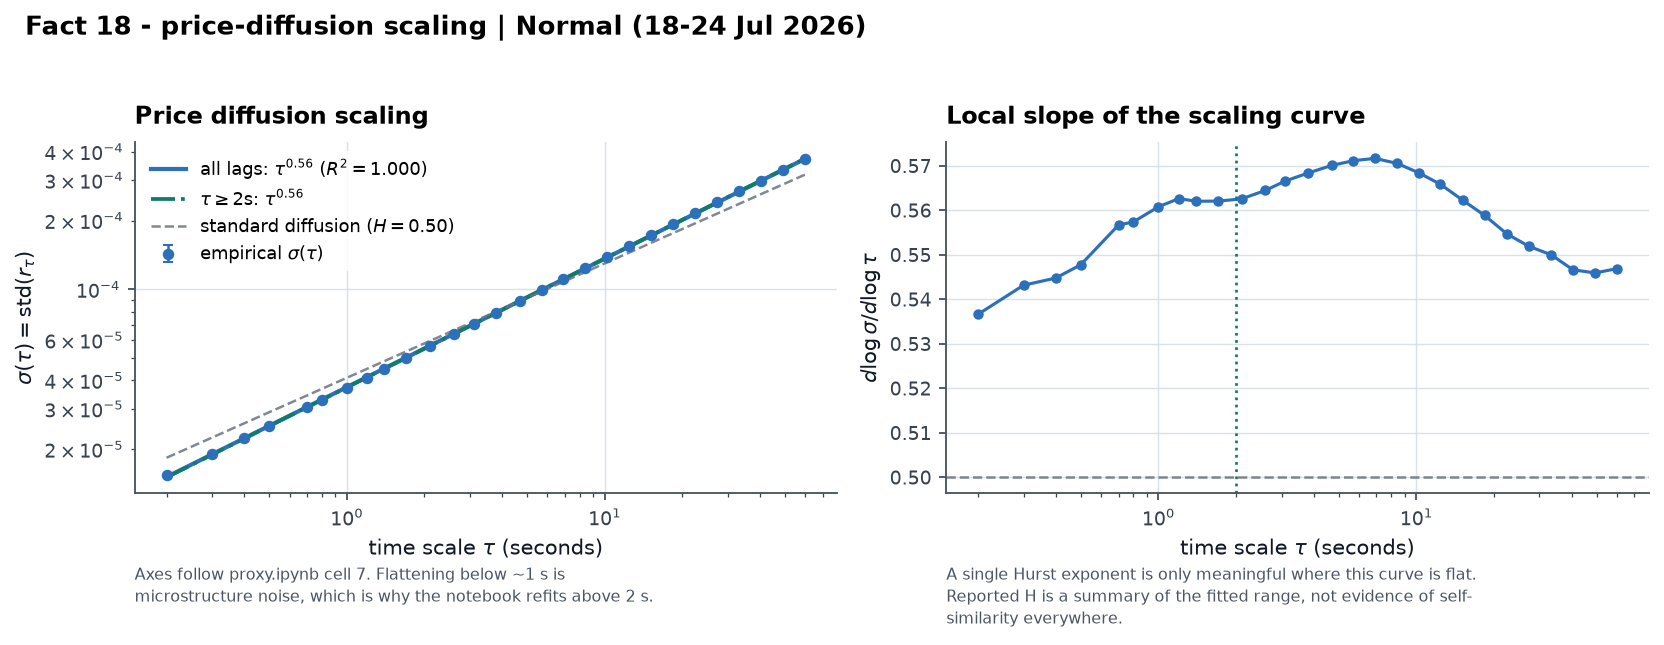
\includegraphics[width=\textwidth,height=0.74\textheight,keepaspectratio]{fact18_volatility_scaling__normal}
\caption{$\sigma(\tau)\sim\tau^{H}$ with $H=0.563$ for $\tau\ge2$\,s, slightly super-diffusive; the
curve flattens below 1\,s where microstructure noise dominates.}
\end{figure}
\end{frame}
\begin{frame}{Fact 22: Order-Timing Regularity}
\begin{figure}
\centering
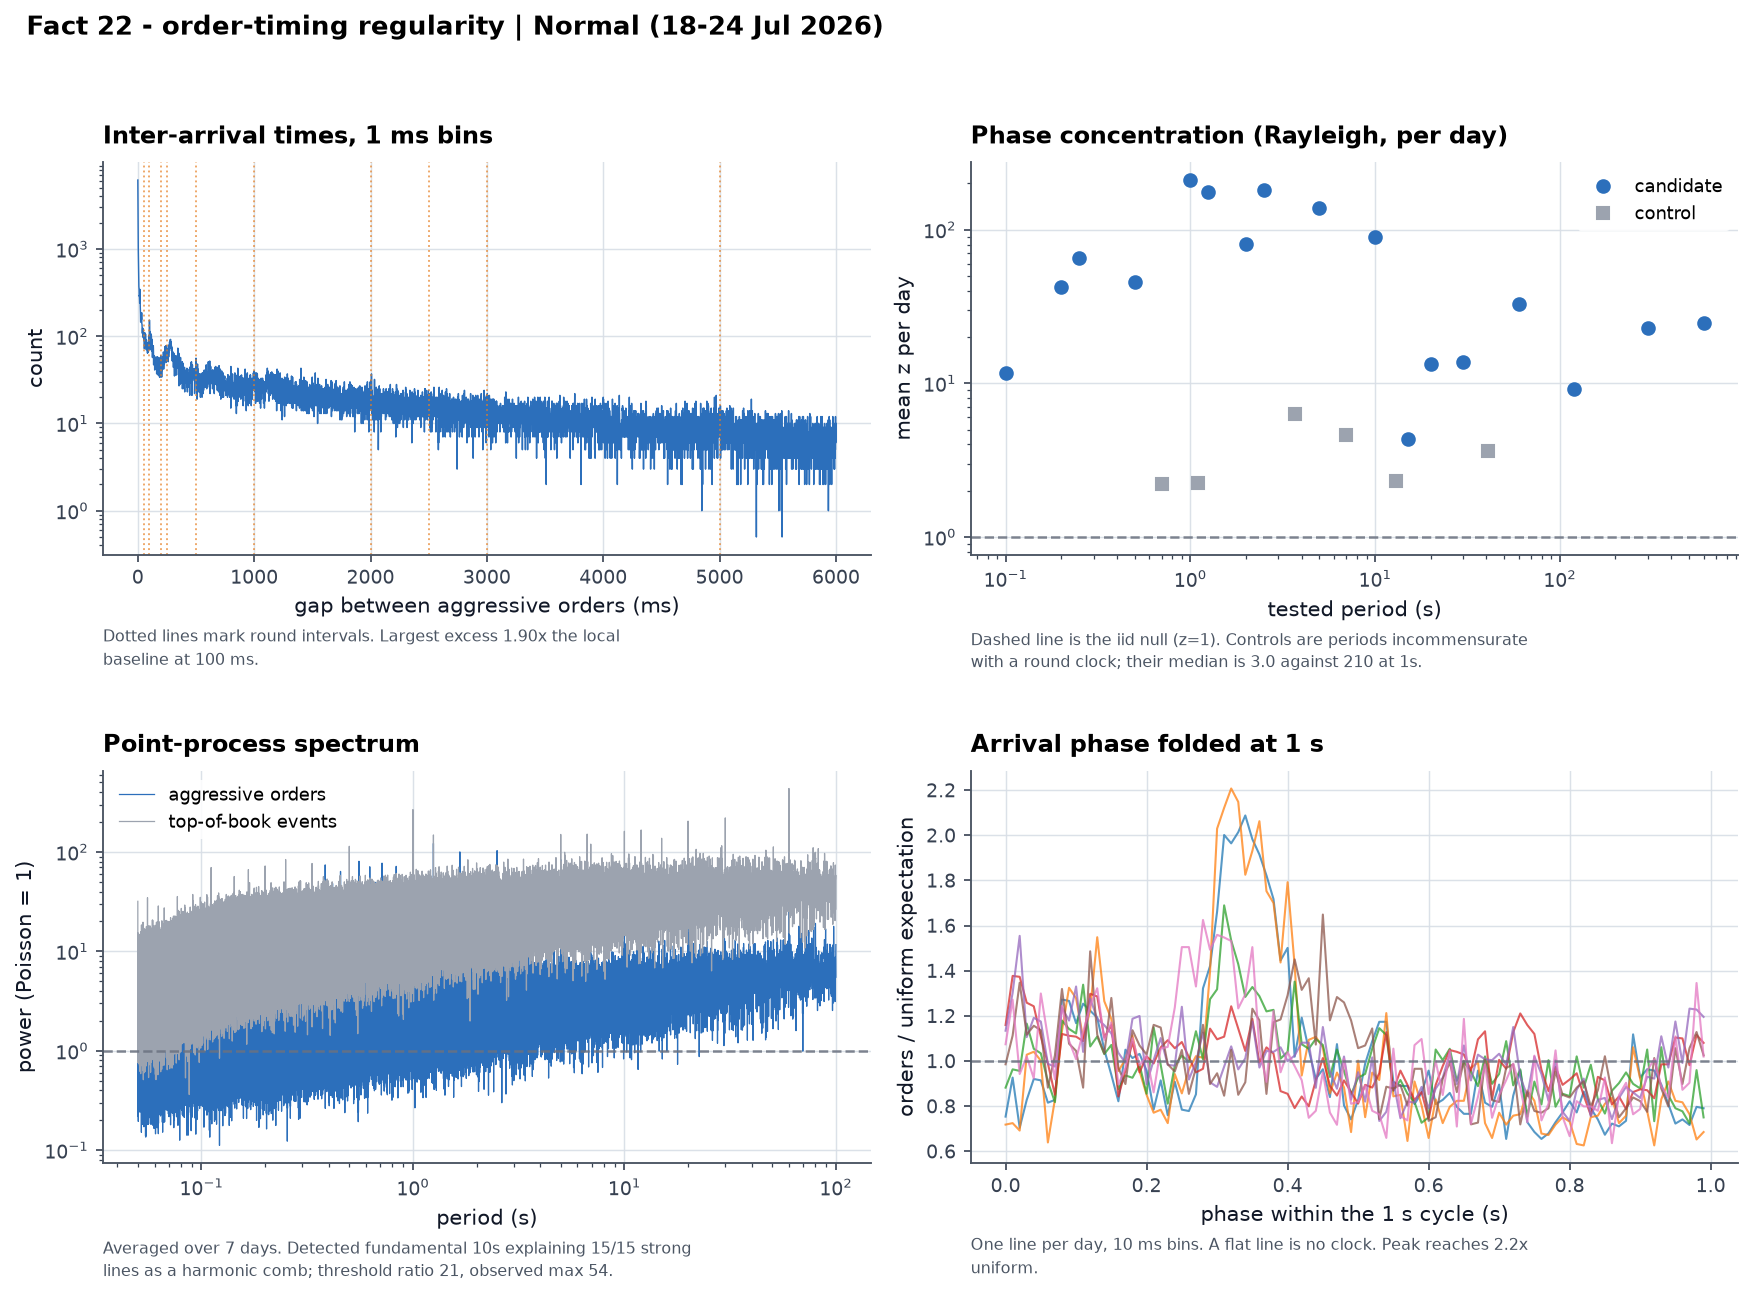
\includegraphics[width=\textwidth,height=0.74\textheight,keepaspectratio]{fact22_order_timing__normal}
\caption{A real execution clock: per-day Rayleigh $z=210$ at 1\,s against incommensurate controls
at 2--6. Every strong spectral line is an exact multiple of 0.1\,Hz, a harmonic comb on a 10\,s
fundamental.}
\end{figure}
\end{frame}
\begin{frame}{Fact 22: Clock Periodicity in the Published Conventions}
\begin{figure}
\centering
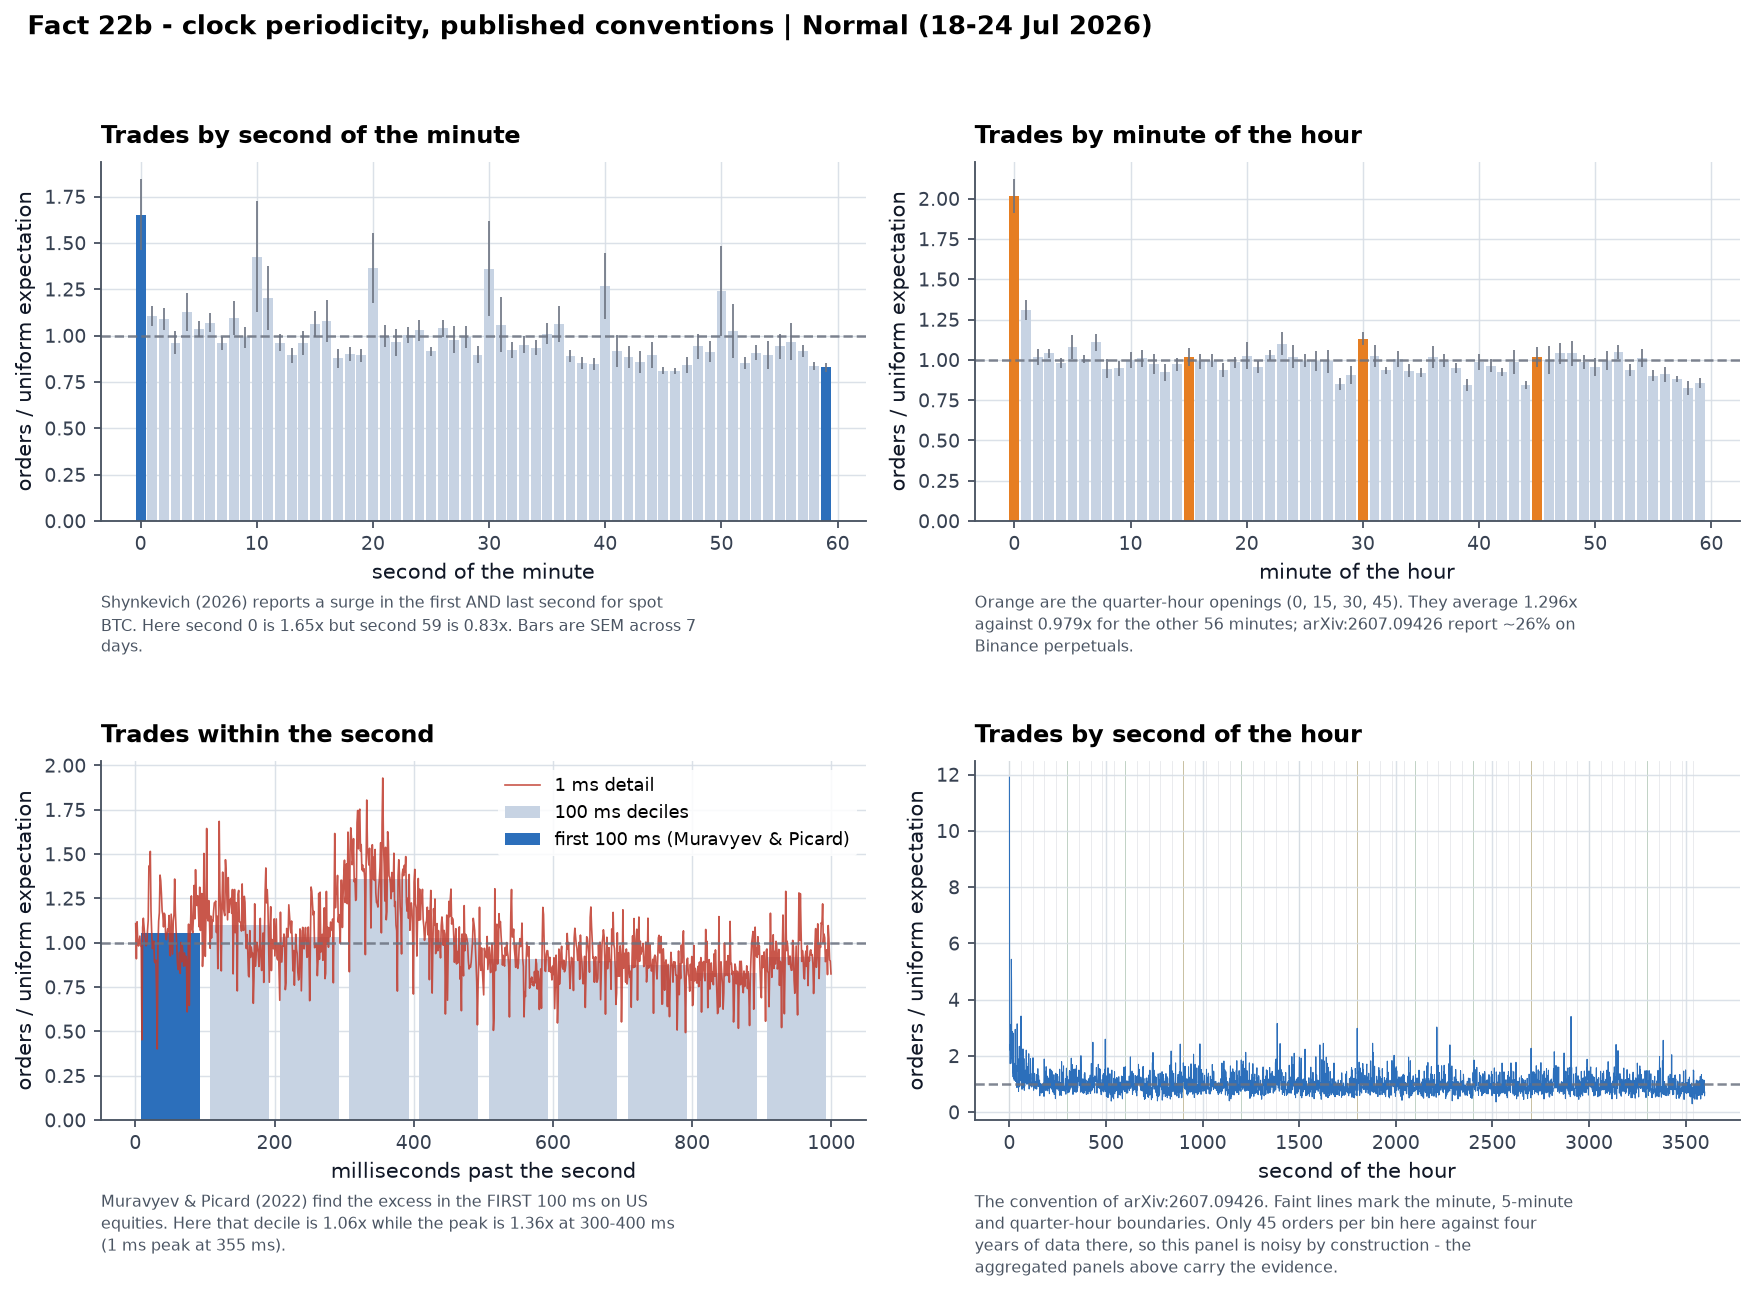
\includegraphics[width=\textwidth,height=0.72\textheight,keepaspectratio]{fact22b_clock_conventions__normal}
\caption{Second 0 of the minute is $1.65\times$ and minute 0 of the hour $2.02\times$ uniform. The
within-second peak sits at 300--400\,ms, not in the first 100\,ms as reported for US equities ---
consistent with transit latency to a non-colocated venue.}
\end{figure}
\end{frame}
\begin{frame}{Fact 17: 24/7 Time-of-Day Structure}
\begin{figure}
\centering

\includegraphics[width=\textwidth,height=0.74\textheight,keepaspectratio]{fact17_time_of_day__normal}
\caption{No equity-style U-shape (edge-to-middle volume ratio 0.62), but hourly volume still varies
by a factor of 5.6 and spread by 2.4.}
\end{figure}
\end{frame}
\begin{frame}{Summary: Normal Week}
\footnotesize
\begin{tabularx}{\textwidth}{@{}L{0.72}L{1.28}@{}}
\toprule
\textbf{Matches the literature} & \textbf{Does not} \\
\midrule
Sign long memory, $\gamma=0.54$ &
Metaorder concavity far below square root: $\delta\approx0.21$--$0.23$ against 0.5 \\
$\mathcal{R}(\ell)$ rising and settling &
Execution trajectory linear, not concave ($0.39$ against $0.71$) \\
Cost rising with size; symmetric book &
OFI dominates trade-flow imbalance ($0.52$ against $0.21$ at 10\,s) \\
Volatility clustering; heavy size tail &
$\mathcal{R}^{+}(1)>\mathcal{R}^{-}(1)$ reverses once the spread faced is controlled \\
Queue imbalance predictive &
No U-shape, but hour-of-day variation is large \\
Over-dispersed arrivals &
Within-second peak at 300--400\,ms, not the first 100\,ms \\
\bottomrule
\end{tabularx}

\medskip
\textbf{Caveat on Facts 1--3.} The proxy assembles parents at random, so a group of six trades is
typically one large trade plus small ones: the median parent holds 66\% of its volume in a single
child. The volume-progress axis is therefore barely resolved, and the linear trajectory should be
read as "not measurable on this instrument", not as a market property.
\end{frame}
\begin{frame}{Implications for the Simulator}
\footnotesize
\begin{tabularx}{\textwidth}{@{}L{0.62}L{1.38}@{}}
\toprule
\textbf{Design choice} & \textbf{What this data says} \\
\midrule
Taker arrival process &
Do not use Poisson. Counts are over-dispersed by 3$\times$ at 1\,s and 28$\times$ at 300\,s, and
interarrivals have a heavy tail. A self-exciting (Hawkes) or burst-and-gap process is the minimum
that reproduces this. \\[3pt]
Taker order sizes &
Heavy-tailed: p99/median $\approx700\times$, and the largest 1\% of orders carry 40\% of volume.
A single characteristic size will understate queue depletion. \\[3pt]
Arrival timing &
Order flow is anchored to the wall clock: second 0 of the minute is $1.65\times$ uniform, minute 0
of the hour $2.02\times$, with a within-second peak at 300--400\,ms. A TWAP child order landing on
the round second meets a crowd. \\[3pt]
Market-maker quoting &
The book is one tick wide 97.6\% of the time but only 80.2\% of updates; wide spreads are
short-lived (16\,ms mean dwell against 164\,ms). Quote width must be modelled in time, not in
events. \\[3pt]
Impact calibration target &
Signed impact is concave but far below square root on this proxy
($\delta\approx0.21$--$0.23$). Do not hard-code $\delta=0.5$; treat it as a parameter and report
the proxy caveat with it. \\[3pt]
Price-flow coupling &
Book-event imbalance dominates trade-flow imbalance ($R^2=0.52$ against $0.21$ at 10\,s), and the
relation peaks near 60\,s. A trades-only impact model leaves most of the explainable move on the
table. \\
\bottomrule
\end{tabularx}
\end{frame}
% =====================================================================
\appendix
% =====================================================================

\begin{frame}[plain]
  \centering
  \vfill
  {\Large\bfseries Appendix}\\[4pt]
  {\normalsize Normal versus Stress Week}\\[10pt]
  {\footnotesize Normal: 18--24 July 2026 \quad$\cdot$\quad Stress: 26 July -- 2 August 2026}\\[2pt]
  {\footnotesize By 31 July, options positioning had turned bearish and spot sold off into month end.}
  \vfill
\end{frame}

\begin{frame}{Reconstruction Validation}
\begin{figure}
\centering

\includegraphics[width=\textwidth,height=0.74\textheight,keepaspectratio]{fact00_reconstruction_validation__compare}
\caption{Reconstructed quotes against the exchange's own snapshot blocks: 107 free out-of-sample
checks across both weeks, median error 0 ticks.}
\end{figure}
\end{frame}

\begin{frame}{Facts 1--3: Metaorder Impact, $N=6$ Proxy}
\footnotesize
\begin{tabularx}{\textwidth}{@{}Xrr@{}}
\toprule
\textbf{Quantity ($N=6$, mean of 3 seeds)} & \textbf{Normal} & \textbf{Stress} \\
\midrule
Parents measured                         & 35{,}834 & 43{,}088 \\
Median children per parent               & 3        & 3 \\
Median duration (s)                      & 30.0     & 27.7 \\
Share with positive signed impact        & 0.556    & 0.610 \\
\midrule
Broken power law $\delta_2$              & 0.212    & 0.196 \\
Single-slope $\delta$                    & 0.230    & 0.216 \\
Prefactor $Y$                            & 0.061    & 0.057 \\
Duration exponent $\gamma$               & 0.247    & 0.201 \\
Volume-clock exponent $\nu$              & 0.194    & 0.118 \\
Decay exponent $\beta$                   & 0.142    & 0.142 \\
Hurst $H$ ($\tau\ge2$\,s)                & 0.563    & 0.567 \\
Trajectory $y(0.5)/y(1)$                 & 0.389    & 0.397 \\
\bottomrule
\end{tabularx}

\medskip
\footnotesize Reported as a table because the per-regime comparison figure is generated only for
the legacy run-based proxy. Seed spread is construction sensitivity on one market sample, not a
confidence interval.
\end{frame}

\newcommand{\comparelide}[3]{%
\begin{frame}{#1}
\begin{figure}
\centering
\includegraphics[width=\textwidth,height=0.74\textheight,keepaspectratio]{#2}
\caption{#3}
\end{figure}
\end{frame}}

\comparelide{Fact 5: Liquidity Cost and Depth}{fact05_liquidity_cost_and_depth__compare}
{Cost and visible depth, normal against stress.}

\comparelide{Fact 6: Spread Distribution}{fact06_spread_distribution__compare}
{Spread widens in the stress week: mean 2.05 ticks against 1.83.}

\comparelide{Fact 7: Liquidity Resiliency}{fact07_resiliency__compare}
{Recovery after large aggressive orders, both regimes.}

\comparelide{Fact 8: Order-Flow Imbalance}{fact08_ofi_response__compare}
{OFI response and its depth dependence.}

\comparelide{Fact 8b: OFI versus TFI}{fact08b_ofi_tfi__compare}
{OFI leads trade-flow imbalance on every horizon and in both regimes.}

\comparelide{Fact 8c: Real-Time OFI}{fact08c_realtime_ofi_tfi__compare}
{$R^2$ peaks near 60\,s in both weeks (0.61 normal, 0.62 stress) and decays beyond.}

\comparelide{Fact 9: Trade Response Function}{fact09_trade_response__compare}
{Response function by regime.}

\comparelide{Fact 9: Conditional Response}{fact09b_conditional_response__compare}
{$\mathcal{R}(\ell)$, $\mathcal{R}(v,1)$ and the sign-conditioned split.}

\comparelide{Fact 10: Order-Sign Long Memory}{fact10_sign_memory__compare}
{Sign autocorrelation: $\gamma=0.54$ normal, $0.43$ stress.}

\comparelide{Fact 11: Diffusivity}{fact11_diffusion__compare}
{Variance ratios and return autocorrelation by regime.}

\comparelide{Fact 12: Selective Liquidity Taking}{fact12_selective_liquidity__compare}
{Pre-trade liquidity around large aggressive orders.}

\comparelide{Fact 13: Queue Imbalance}{fact13_queue_imbalance__compare}
{Queue-imbalance predictability by regime.}

\comparelide{Fact 14: Volatility Clustering}{fact14_volatility_clustering__compare}
{Absolute-return autocorrelation by regime.}

\comparelide{Fact 16: Trade-Size Distribution}{fact16_trade_size__compare}
{Aggressive-order and fill size distributions.}

\comparelide{Fact 17: Time-of-Day Structure}{fact17_time_of_day__compare}
{Hourly volume, spread and depth profiles.}

\comparelide{Fact 18: Price-Diffusion Scaling}{fact18_volatility_scaling__compare}
{$H=0.563$ normal against $0.567$ stress.}

\comparelide{Fact 19: Event Arrivals}{fact19_arrivals__compare}
{Interarrival distributions and count dispersion.}

\comparelide{Fact 20: Book Shape}{fact20_book_shape__compare}
{Tick spread and depth-per-tick profile by regime.}

\comparelide{Fact 22: Order-Timing Regularity}{fact22_order_timing__compare}
{Phase concentration and point-process spectrum, both weeks.}

\comparelide{Fact 22: Clock Periodicity}{fact22b_clock_conventions__compare}
{Second-of-minute and within-second profiles by regime.}

% =====================================================================
\begin{frame}[allowframebreaks]{References}
\footnotesize
\begin{thebibliography}{99}

\bibitem{bacry2015}
E.~Bacry, I.~Mastromatteo, J.-F.~Muzy (2015).
\newblock Hawkes processes in finance.
\newblock \emph{Market Microstructure and Liquidity} 1(1).

\bibitem{bouchaud2004}
J.-P.~Bouchaud, Y.~Gefen, M.~Potters, M.~Wyart (2004).
\newblock Fluctuations and response in financial markets: the subtle nature of `random' price changes.
\newblock \emph{Quantitative Finance} 4(2), 176--190.
\newblock \href{https://arxiv.org/abs/cond-mat/0307332}{arXiv:cond-mat/0307332}

\bibitem{byrd2020}
D.~Byrd, M.~Hybinette, T.~H.~Balch (2020).
\newblock ABIDES: towards high-fidelity multi-agent market simulation.
\newblock \emph{ACM SIGSIM-PADS}.

\bibitem{cont2001}
R.~Cont (2001).
\newblock Empirical properties of asset returns: stylized facts and statistical issues.
\newblock \emph{Quantitative Finance} 1(2), 223--236.

\bibitem{cont2014}
R.~Cont, A.~Kukanov, S.~Stoikov (2014).
\newblock The price impact of order book events.
\newblock \emph{Journal of Financial Econometrics} 12(1), 47--88.
\newblock \href{https://arxiv.org/abs/1011.6402}{arXiv:1011.6402}

\bibitem{donier2015}
J.~Donier, J.~Bonart (2015).
\newblock A million metaorder analysis of market impact on the Bitcoin.
\newblock \emph{Market Microstructure and Liquidity} 1(2).
\newblock \href{https://arxiv.org/abs/1412.4503}{arXiv:1412.4503}

\bibitem{gould2016}
M.~D.~Gould, J.~Bonart (2016).
\newblock Queue imbalance as a one-tick-ahead price predictor in a limit order book.
\newblock \emph{Market Microstructure and Liquidity} 2(2).
\newblock \href{https://arxiv.org/abs/1512.03492}{arXiv:1512.03492}

\bibitem{jain2024}
K.~Jain, N.~Firoozye, J.~Kochems, P.~Treleaven.
\newblock Limit order book simulations: a review.

\bibitem{lillo2004}
F.~Lillo, J.~D.~Farmer (2004).
\newblock The long memory of the efficient market.
\newblock \emph{Studies in Nonlinear Dynamics \& Econometrics} 8(3).
\newblock \href{https://arxiv.org/abs/cond-mat/0311053}{arXiv:cond-mat/0311053}

\bibitem{lo1988}
A.~W.~Lo, A.~C.~MacKinlay (1988).
\newblock Stock market prices do not follow random walks: evidence from a simple specification test.
\newblock \emph{Review of Financial Studies} 1(1), 41--66.
\newblock \href{https://academic.oup.com/rfs/article/1/1/41/1601244}{academic.oup.com/rfs/1/1/41}

\bibitem{maitrier2025a}
G.~Maitrier, G.~Loeper, J.-P.~Bouchaud (2025a).
\newblock Generating realistic metaorders from public data.
\newblock \href{https://arxiv.org/abs/2503.18199}{arXiv:2503.18199}

\bibitem{maitrier2025b}
G.~Maitrier, G.~Loeper, J.-P.~Bouchaud (2025b).
\newblock The subtle interplay between square-root impact, order imbalance and volatility II:
an artificial market generator.
\newblock \href{https://arxiv.org/abs/2509.05065}{arXiv:2509.05065}

\bibitem{muravyev2022}
D.~Muravyev, J.~Picard (2022).
\newblock Does trade clustering reduce trading costs? Evidence from periodicity in algorithmic trading.
\newblock \emph{Financial Management} 51(4).
\newblock \href{https://onlinelibrary.wiley.com/doi/10.1111/fima.12405}{doi:10.1111/fima.12405}

\bibitem{obizhaeva2013}
A.~A.~Obizhaeva, J.~Wang (2013).
\newblock Optimal trading strategy and supply/demand dynamics.
\newblock \emph{Journal of Financial Markets} 16(1), 1--32.

\bibitem{schnaubelt2019}
M.~Schnaubelt, J.~Rende, C.~Krauss (2019).
\newblock Testing stylized facts of Bitcoin limit order books.
\newblock \emph{Journal of Risk and Financial Management} 12(1), 25.
\newblock \href{https://www.mdpi.com/1911-8074/12/1/25}{mdpi.com/1911-8074/12/1/25}

\bibitem{shynkevich2026}
A.~Shynkevich (2026).
\newblock When the clock strikes: algorithmic trading in cryptocurrency markets.
\newblock \emph{Applied Economics Letters}.
\newblock \href{https://www.tandfonline.com/doi/full/10.1080/13504851.2026.2617499}{doi:10.1080/13504851.2026.2617499}

\bibitem{webster2023}
K.~Webster (2023).
\newblock \emph{Handbook of Price Impact Modeling}.
\newblock Chapman \& Hall/CRC.

\end{thebibliography}
\end{frame}

\end{document}